\begin{frame}[fragile]{GNU Radio Installation (7/7)}

\textbf{\textcolor{red}{NEEL FIXME (remove Soapy)}}

\footnotesize

\begin{itemize}
    \item \textbf{Verify the SoapySDR Installation.}

    \begin{itemize}
        \item SoapySDR is a vendor-independent hardware abstraction library that
        provides a common API to interface with different Software Defined Radio
        (SDR) devices through hardware-specific drivers.
    \end{itemize}
\end{itemize}

\scriptsize

\begin{Verbatim}[xleftmargin=2.8em,breaklines,breaksymbolleft={},breaksymbolright={}]
# SoapySDR library
SoapySDRUtil --info
\end{Verbatim}



\begin{center}
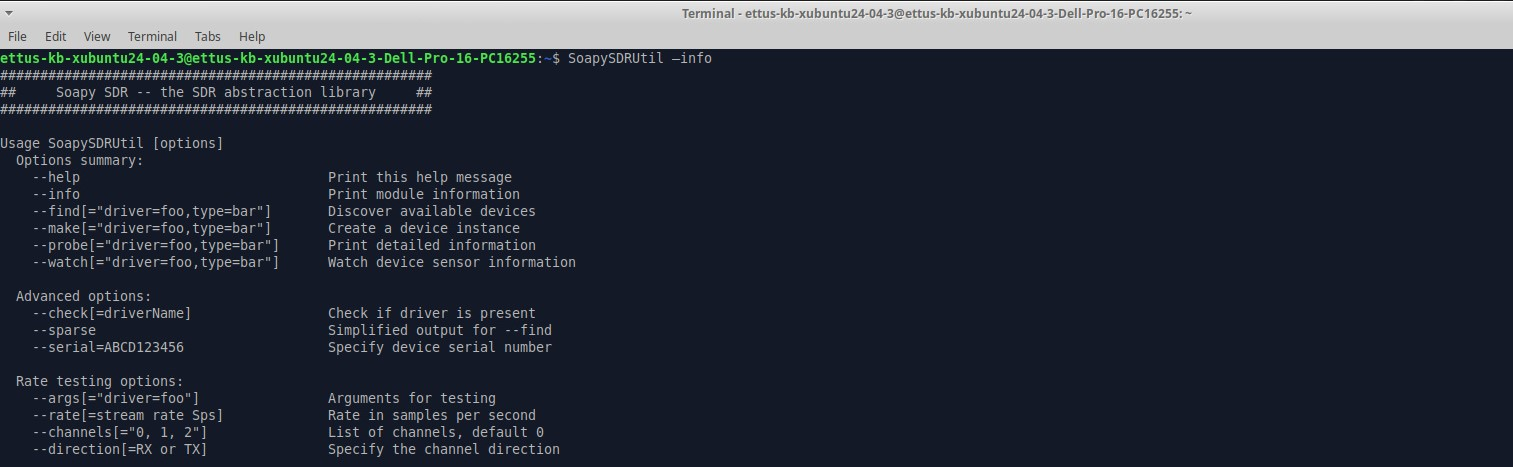
\includegraphics[width=0.8\linewidth]{latex/jpg_png/image_soapy sdr output.jpg}
\end{center}

\end{frame}